\newpage
\chapter{Interfacing a model with the PSMILe library}
\label{sec_modelinterfacing}

At run-time, OASIS3 acts as a separate mono process executable which
drives the coupled run, interpolates and transforms the coupling
fields. To communicate with OASIS3 or directly between the component
models, different communication techniques have been historically
developed. The technique used for one particular run is defined by the
user in the configuration file {\it namcouple} (see section
\ref{sec_namcouple}). In OASIS3, the CLIM communication technique
based on MPI1 or MPI2 message passing and the associated model
interface library PSMILe, should be used\footnote{The SIPC, PIPE and
  GMEM communication techniques available in previous versions should
  still work but are not maintained anymore and were not tested.}. For
a practical toy model using the PSMILe library, see the sources in
{\tt /prism/src/mod/toyatm, /toyche, /toyoce} and more details in
chapter \ref{sec_compilationrunning}.


%\vspace*{0.5cm}

 To communicate with OASIS3 or directly with another component model
 using the CLIM-MPI1/2 communication technique,
  or to perform I/O actions, a component model needs to be interfaced
  with the PRISM System Model Interface library, PSMILe, which sources
  can be found in {\tt prism/src/lib/psmile} directory. PSMILe supports:

\begin{itemize}
\item parallel communication between a parallel component
 model and OASIS3 main process,
\item direct communication between two parallel component models when no
 transformations and no repartitioning are required,
\item automatic sending and receiving actions at appropriate times
 following user's choice indicated in the {\it namcouple},
\item time integration or accumulation of the coupling fields,
\item I/O actions from/to files.
\end{itemize}

 To adapt a component model to PSMILe, specific calls of
 the following classes have to be implemented in the code:

\begin{enumerate}
\item Initialisation (section \ref{subsubsec_Initialisation})
\item Grid data file definition (section \ref{subsubsec_griddef})
\item Partition definition (section \ref{subsubsec_Partition})
\item I/O-coupling field declaration (section \ref{subsubsec_Declaration})
\item End of definition phase (section \ref{subsubsec_Endofdefinition})
\item I/O-coupling field sending and receiving (section
\ref{subsubsec_sendingreceiving})
\item Termination (section \ref{subsubsec_Termination})
\end{enumerate}

Finally, in section \ref{subsubsec_Algoritms}, different coupling
algorithms are illustrated, and explanations are given on how to
reproduce them with PSMILe by defining the appropriate indices of
lag and sequence for each coupling field.

\section{Initialisation}
\label{subsubsec_Initialisation}
%{Initialisation}

All processes of the component model initialise the coupling and, if
required, retrieve a local communicator for the component model
internal parallelisation.

\begin{itemize}

\item {\tt USE mod\_prism\_proto}
 
Module to be used by the component models. 

\item {\tt CALL prism\_init\_comp\_proto (compid, model\_name, ierror)} 

 \begin{itemize}
   \item {\tt compid [INTEGER; OUT]}: component model ID 
   \item {\tt model\_name [CHARACTER*6; IN]}: name of calling model (as in
  {\em namcouple}) 
   \item {\tt ierror [INTEGER; OUT]}: returned error code.
 \end{itemize}
 
Routine called by all component model processes, which initialises the
coupling.\footnote{The model may call MPI\_Init explicitly, but if so, has to
call it before calling {\tt prism\_init\_comp\_proto}; in this case, the
model also has to call MPI\_Finalize explicitly, but only after calling
{\tt prism\_terminate\_proto}.}

\item {\tt CALL prism\_get\_localcomm\_proto (local\_comm, ierror )}

 \begin{itemize}
   \item {\tt local\_comm [INTEGER; OUT]}: value of local communicator
   \item {\tt ierror [INTEGER; OUT]}: returned error code.
  \end{itemize}

  For CLIM-MPI1 communication technique: routine called by all model
  processes to get the value of a local communicator to be used by the
  model for its internal parallelisation.

  In fact, with CLIM-MPI1, all component models started in a
  pseudo-MPMD mode share automatically the same MPI\_COMM\_WORLD
  communicator.  Another communicator has to be used for the internal
  parallelisation of each model. OASIS3 creates this model local
  communicator following a ``coloring scheme"; its value is returned
  as the first argument of prism\_get\_localcomm\_proto routine.

  With CLIM-MPI2, the communicator MPI\_COMM\_WORLD will be returned as
  local communicator.

  Besides that, the differences between using PSMILe with MPI1 or MPI2
  message passing are
  \begin{itemize}
  \item The \$CHANNEL in the namcouple; see section
    \ref{subsec_namcouplefirst}.
  \item The way the models are started. With MPI2, only OASIS3 needs
    to be started at the command line; it will then spawn the
    component models at the beginning of the run.  With MPI1, models
    have to be started by the user in a pseudo-MPMD mode; the way to
    do this depends on the computing platform. For more details, see
    section \ref{subsec_running}.
  \end{itemize}
\end{itemize}

\section{Grid data file definition}
\label{subsubsec_griddef}

The grid data files {\em grids.nc, masks.nc} and {\em areas.nc} must
be created by the user before the run or can be written directly
at run time by the master process of each component model. 

If written by the component models, the writing of those grid files is
driven by OASIS3 main process. It first checks whether the binary file
{\em grids} or the netCDF file {\em grids.nc} exists (in that case, it
is assumed that {\em areas} or {\em areas.nc} and {\em masks} or {\em
masks.nc} files exist too), or if writing is needed. If {\em grids} or
{\em grids.nc} exists, it must contain all grid information from all
models; if it does not exist, each model must write its grid
definition in the grid data files.

The coupler sends the information on whether or not writing is needed
to the mo\-dels following an OASIS internal order (below
prism\_start\_grids\_writing). If no writing is needed, nothing
happens when calling the following prism\_write\_xxxx routines. If
writing is needed, the first model creates the files, writes the data
arrays (with {\tt prism\_write\_grid}, {\tt prism\_write\_corner},
{\tt prism\_write\_mask}, {\tt prism\_write\_area} calls),
and then sends a termination flag to the coupler (below \break {\tt
prism\_terminate\_grids\_writing} call). The coupler will send the
starting flag to the next model; this ensures that only one model
accesses the files at a time.

This section describes the PSMILe routines that may be called by the
master process of each component model to write, at run time, the whole
grid information to the grid data files. These routines have to
be called just after {\tt prism\_init\_comp\_proto}.

The TOYCLIM coupled model 
uses those routines to write its grid data
files if \texttt{gridswr=1} in the running script
\texttt{run\_toyclim}  
%XXXXX or \texttt{RUN\_toyclim\_$<$expid$>$} 
(see section \ref{subsec_running}).

%To run a toy experiment
%into which the component models write those files, execute the
%script prism/util/running/toyclim/sc\_run\_toyclim\_grid. 

\begin{itemize}
\item {\tt USE  mod\_prism\_grids\_writing}

Module to be used by the component model to call grid writing routines.
  
\item {\tt CALL  prism\_start\_grids\_writing (flag)}
        
  \begin{itemize}
    \item {\tt flag [INTEGER; OUT]}:  returns 1/0 if grids writing is
    needed/not needed
  \end{itemize}
Initialisation of grids writing.

\item {\tt CALL prism\_write\_grid (cgrid, nx, ny, lon, lat)}
        
 \begin{itemize}
    \item {\tt cgrid [CHARACTER*4; IN]}: grid name prefix (see
    \ref{subsec_namcouplesecond}
    \item {\tt nx [INTEGER; IN]} : grid dimension in x-direction
    \item {\tt ny [INTEGER; IN]} : grid dimension in y-direction
    \item {\tt lon [REAL, DIMENSION(nx,ny); IN)} : array of longitudes
      (degrees East) 
    \item {\tt lat [REAL, DIMENSION(nx,ny); IN)} : array of latitudes
    (degrees North)
 \end{itemize}

 Writing of the model grid longitudes and latitudes. Longitudes must
 be given in degrees East in the interval -360.0 to 720.0. Latitudes
 must be given in degrees North in the interval -90.0 to 90.0. Note
 that if some grid points overlap, it is recommended to define those
 points with the same number (e.g. 90.0 for both, not 450.0 for one
 and 90.0 for the other) to ensure automatic detection of overlap by OASIS
 (which is essential to have a correct conservative remapping
 \texttt{SCRIPR/CONSERV}, see section \ref{subsec_interp}). 


\item {\tt CALL prism\_write\_corner (cgrid, nx, ny, nc, clon, clat)}

 \begin{itemize}
    \item {\tt cgrid [CHARACTER*4; IN]}: grid name prefix
    \item {\tt nx [INTEGER; IN]} : grid dimension in x-direction
    \item {\tt ny [INTEGER; IN]} : grid dimension in y-direction
    \item {\tt nc [INTEGER; IN]} : number of corners per grid cell (4)
    \item {\tt lon [REAL, DIMENSION (nx,ny,nc);IN]} : array of corner
    longitudes (in degrees\_East)
    \item {\tt lat [REAL, DIMENSION (nx,ny,nc);IN]} : array of corner
    latitudes (in degrees\_North)
 \end{itemize}

 Writing of the grid cell corner longitudes and latitudes
 (counterclockwise sense). Longitudes must be given in degrees East in
 the interval -360.0 to 720.0. Latitudes must be given in degrees
 North in the interval -90.0 to 90.0. Note also that cells larger than
 180.0 degrees in longitude are not supported. Writing of corners is
 optional as corner information is needed only for some
 transformations (see section \ref{subsec_griddata}). If called,
 prism\_write\_corners needs to be called after prism\_write\_grids.

\item {\tt CALL prism\_write\_mask (cgrid, nx, ny, mask)}
 \begin{itemize}
    \item {\tt cgrid [CHARACTER*4; IN]}: grid name prefix 
    \item {\tt nx [INTEGER; IN]} : grid dimension in x-direction
    \item {\tt ny [INTEGER; IN]} : grid dimension in y-direction
    \item {\tt mask [INTEGER, DIMENSION(nx,ny) ;IN]} : mask array (0 - not masked, 1 - masked)
 \end{itemize}
Writing of the model grid mask.

\item {\tt CALL prism\_write\_area (cgrid, nx, ny, area)}
 \begin{itemize}
    \item {\tt cgrid [CHARACTER*4; IN]}: grid name prefix
    \item {\tt nx [INTEGER; IN]} : grid dimension in x-direction
    \item {\tt ny [INTEGER; IN]} : grid dimension in y-direction
    \item {\tt area [REAL, DIMENSION(nx,ny); IN]} : array of grid cell areas
 \end{itemize}
Writing of the model grid cell areas. Writing of areas is optional as
area information is needed only for some transformations (see section
\ref{subsec_griddata}).

\item {\tt CALL prism\_terminate\_grids\_writing()}

Termination of grids writing. A flag stating that all needed grid
information was written will be sent to OASIS3 main process.

\end{itemize}

\section{Partition definition}
\label{subsubsec_Partition}

When a component of the coupled system is a parallel code, each
coupling field is usually scattered among the different
processes. With the PSMILe library, each process sends
directly its partition to OASIS3 main process, or directly to the
other component model if no transformation nor repartition is
required.  To do so, each process implied in the coupling has to
define its local partition in the global index space.

\begin{itemize}

\item {\tt USE mod\_prism\_def\_partition\_proto}

Module to be used by the component model to call {\tt
  prism\_def\_partition\_proto}.

\item {\tt CALL prism\_def\_partition\_proto (il\_part\_id,
   ig\_paral, ierror)}
   \begin{itemize}
   \item {\tt il\_part\_id [INTEGER; OUT]}: partition ID 
   \item {\tt ig\_paral [INTEGER, DIMENSION(:), IN]}: vector of
   integers describing the local partition in the global index space
   \item {\tt ierror [INTEGER; OUT]}: returned error code.
   \end{itemize}
\end{itemize} 

The vector of integers describing the process local partition, {\tt
ig\_paral}, has a different expression depending on the type of the
partition. In OASIS3, 4 types of partition are supported: Serial (no
partition), Apple, Box, and Orange.
 
\subsection{Serial (no partition)}

This is the choice for a monoprocess model. In this case, we have 
{\tt ig\_paral(1:3)}:
\begin{itemize}
 \item {\tt ig\_paral(1)} = 0 (indicates a Serial ``partition'')
 \item {\tt ig\_paral(2)} = 0
 \item {\tt ig\_paral(3)} = the total grid size.
\end{itemize}

\subsection{Apple partition} 

Each partition is a segment of the global domain, described by its
global offset and its local size. In this case, we have {\tt
ig\_paral(1:3)}:
\begin{itemize}
 \item {\tt ig\_paral(1)} = 1 (indicates an Apple partition)
 \item {\tt ig\_paral(2)} = the segment global offset
 \item {\tt ig\_paral(3)} = the segment local size
\end{itemize}

Figure \ref{apple_partition} illustrates an Apple partition over 3
processes.
\begin{figure}
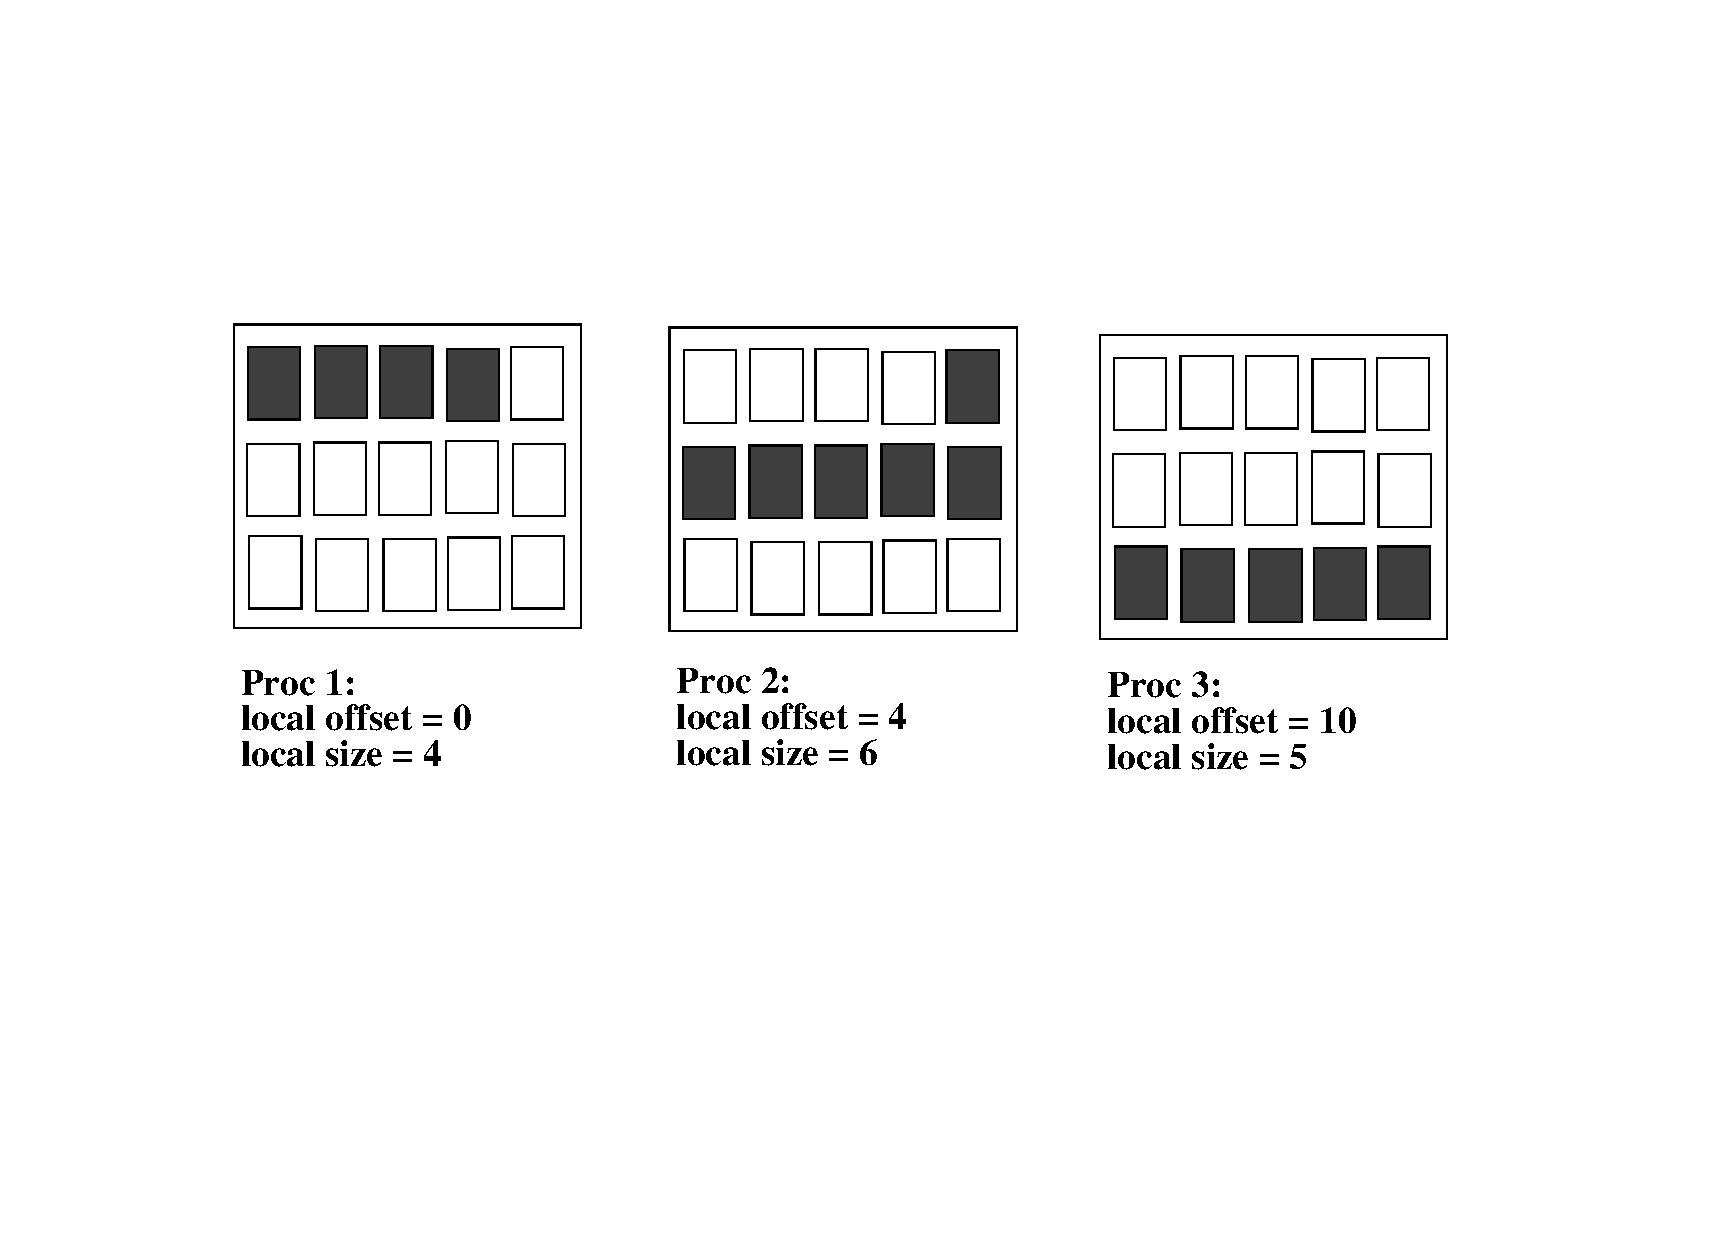
\includegraphics[scale=.6]{apple_new.eps} 
\caption{Apple partition}
\label{apple_partition}
\end{figure}


\subsection{Box partition} 

Each partition is a rectangular region of the global domain, described
by the global offset of its upper left corner, and its local extents in the
X and Y dimensions. The global extent in the X dimension must also be
given. In this case, we have {\tt ig\_paral(1:5)}:
\begin{itemize}
 \item {\tt ig\_paral(1)} = 2 (indicates a Box partition)
 \item {\tt ig\_paral(2)} = the upper left corner global offset
 \item {\tt ig\_paral(3)} = the local extent in X
 \item {\tt ig\_paral(4)} = the local extent in Y\footnote{The maximum
value of the local extent in Y is presently 338; it can be increased
by modifying the value of {\tt Clim\_MaxSegments} in {\tt
prism/src/lib/clim/src/mod\_clim.F90} and in {\tt
prism/src/lib/psmile/src/mod\_prism\_proto.F90} and by recompiling
Oasis3 and the PSMILe library.}
 \item {\tt ig\_paral(5)} = the global extent in X.
\end{itemize}

Figure \ref{box_partition} illustrates a Box partition over 3
processes.  
 
\begin{figure}
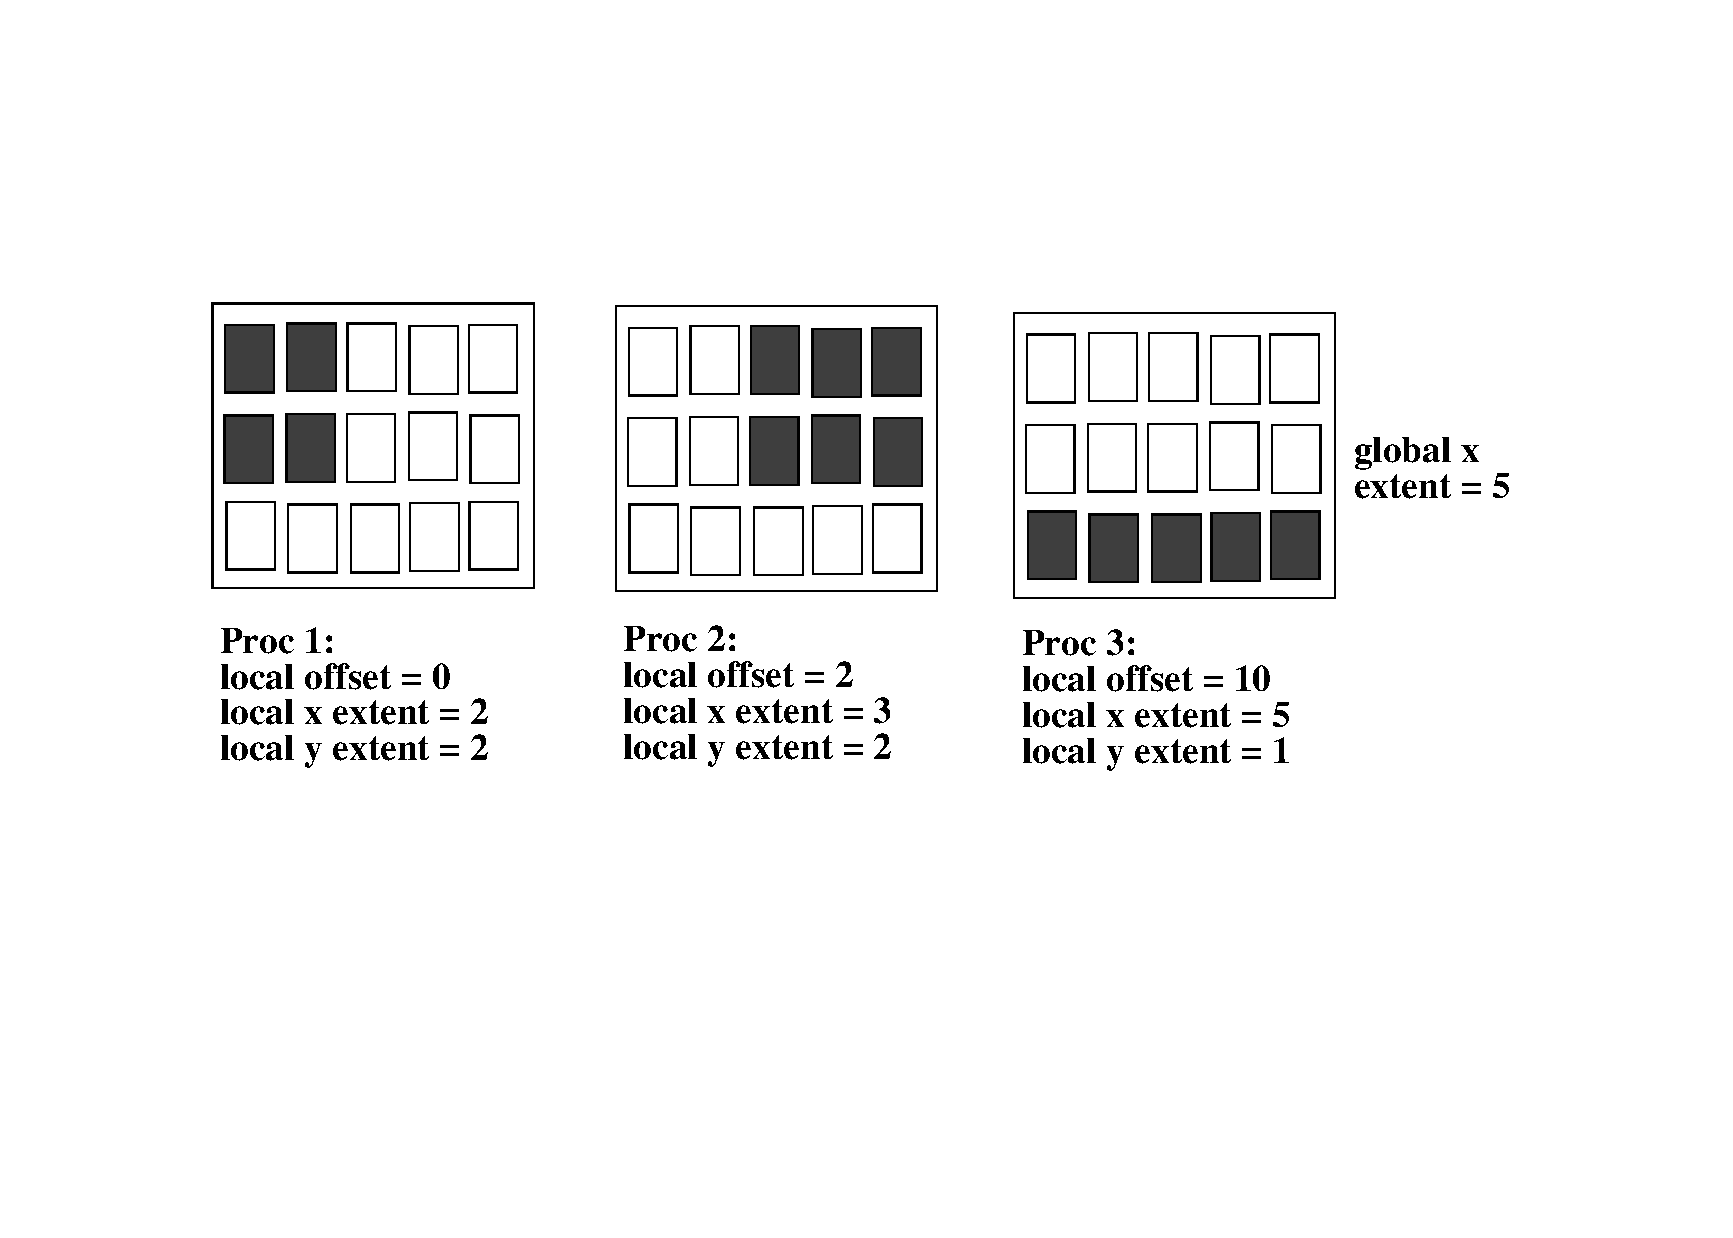
\includegraphics[scale=.6]{box_new.eps} 
\caption{Box partition}
\label{box_partition}
\end{figure} 
  
\subsection{Orange partition}

Each partition is an ensemble of segments of the global domain. Each
segment is described by its global offset and its local extent.  In
this case, we have {\tt ig\_paral(1:N)} where {\tt N = 2 + 2*number of
segments}\footnote{As for the Box partition, the maximum number of
segments is presently 338; it can be increased by modifying the value
of {\tt Clim\_MaxSegments}}.

\begin{itemize}
 \item {\tt ig\_paral(1)} = 3 (indicates a Orange partition)
 \item {\tt ig\_paral(2)} = the total number of segments for the partition (limited to 200 presently, see note for ig\_paral(4) for Box partition above)
 \item {\tt ig\_paral(3)} = the first segment global offset
 \item {\tt ig\_paral(4)} = the first segment local extent
 \item {\tt ig\_paral(5)} = the second segment global offset
 \item {\tt ig\_paral(6)} = the second segment local extent
 \item ...
 \item {\tt ig\_paral(N-1)} = the last segment global offset
 \item {\tt ig\_paral(N)} = the last segment local extent
\end{itemize}

Figure \ref{orange_partition} illustrates an Orange partition with 3 segments
for one process. The other process partitions are not illustrated.

\begin{figure}
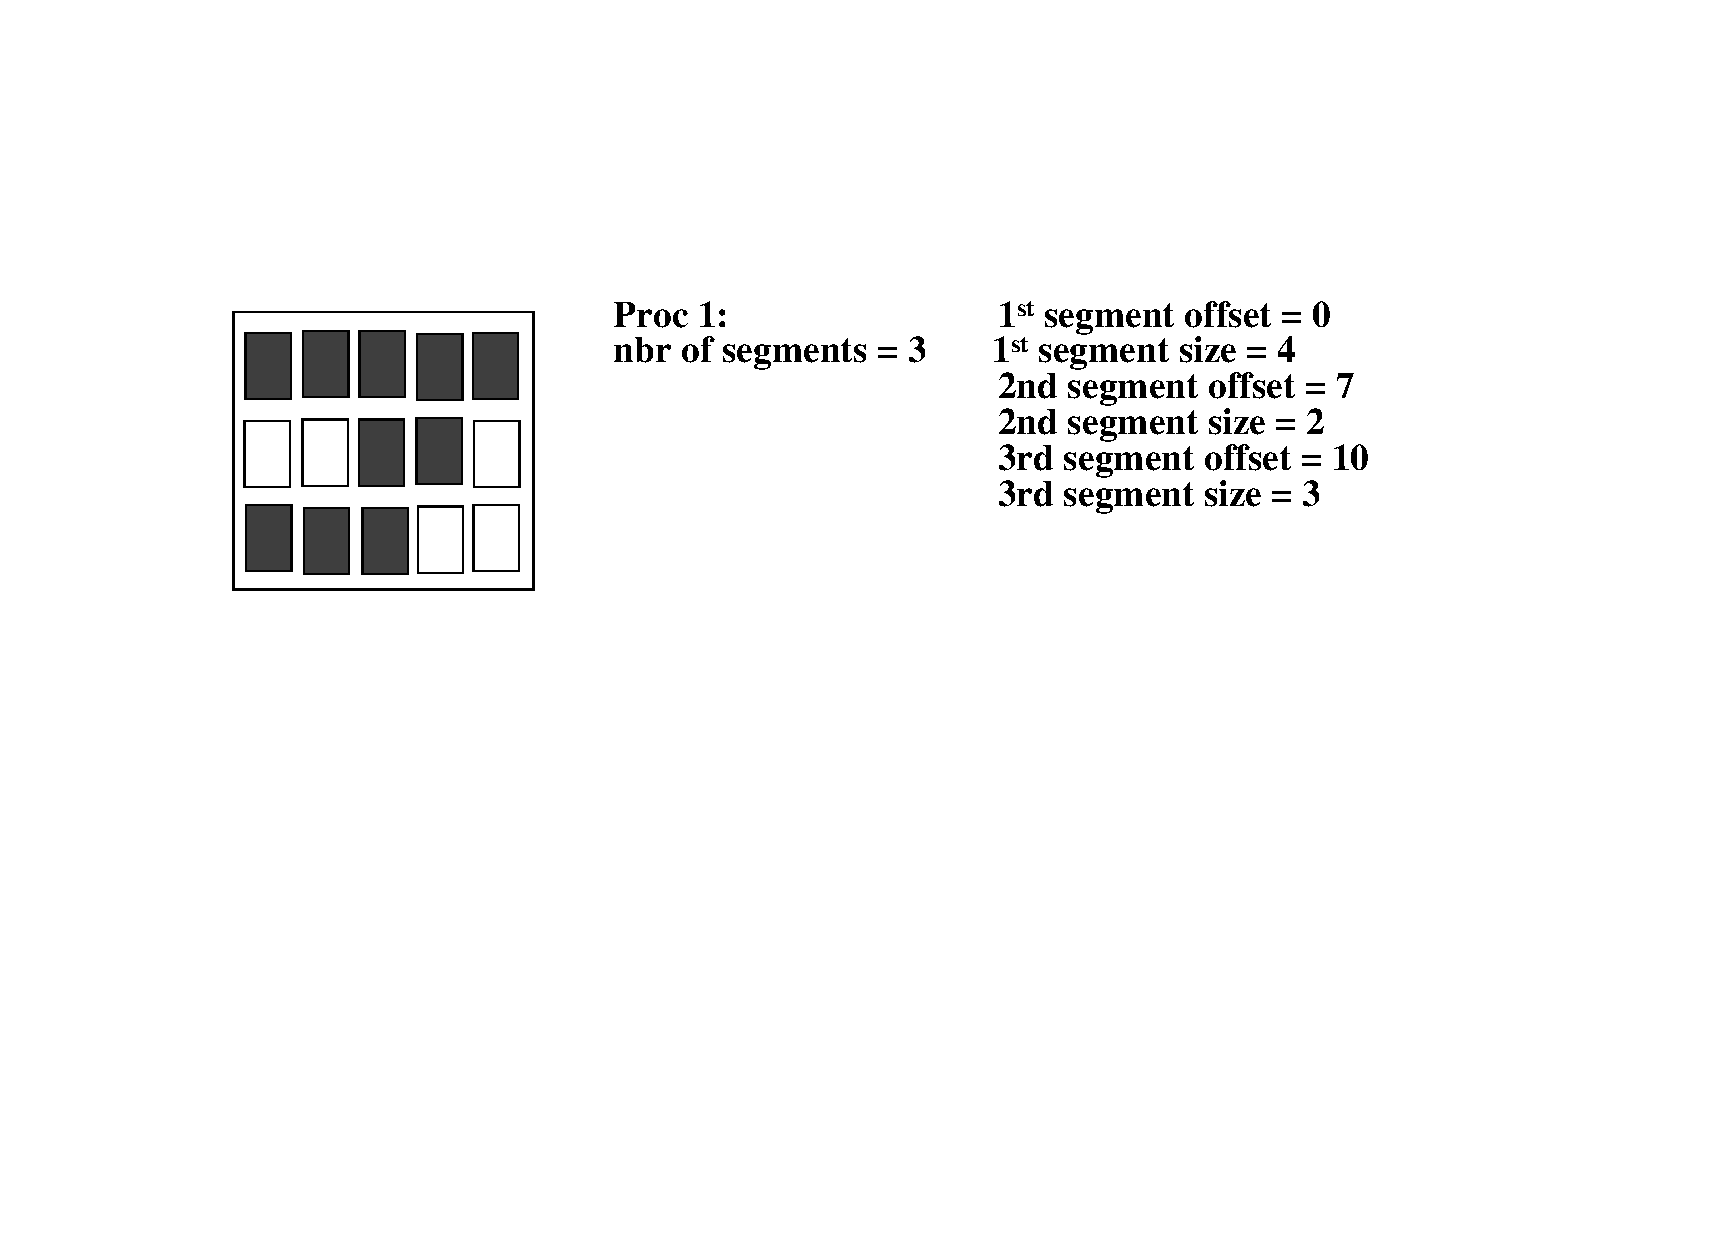
\includegraphics[scale=.6]{orange_new.eps} 
\caption{Orange partition for one process}
\label{orange_partition}
\end{figure} 

%{Partition definition}

\section{I/O-coupling field declaration}
 \label{subsubsec_Declaration}

Each process implied in the coupling declares each field it will send
or receive during the simulation. 

\begin{itemize}

\item {\tt CALL prism\_def\_var\_proto(var\_id, name, il\_part\_id,
  var\_nodims, kinout, var\_actual\_shape, var\_type, ierror)}

\begin{itemize}
 \item {\tt var\_id [INTEGER; OUT]}: coupling field ID
 \item {\tt name [CHARACTER*8; IN]}: field symbolic name (as in the
   {\it namcouple})
 \item {\tt il\_part\_id [INTEGER; IN]}: partition ID (returned by
   {\tt prism\_def\_partition\-\_proto})
 \item {\tt var\_nodims [INTEGER, DIMENSION(2); IN]}: var\_nodims(1) is
   the rank of field array (1 or 2); var\_nodims(2) is the number of
   bundles (always 1 for OASIS3). 
 \item {\tt kinout [INTEGER; IN]}: {\tt PRISM\_In} for fields received by
   the model, or {\tt PRISM\_Out} for fields sent by the model 
 \item {\tt var\_actual\_shape [INTEGER, DIMENSION(2*var\_nodims(1)); IN]}: 
   vector of integers giving the minimum and maximum index for each
   dimension of the coupling field array; for OASIS3, the minimum
   index has to be 1 and the maximum index has to be the extent of the
   dimension.
 \item {\tt var\_type [INTEGER; IN]}: type of coupling field array;
   put {\tt PRISM\_Real} for single or double precision real
   arrays\footnote{PRISM standard is to exchange coupling fields
   declared {\tt REAL(kind=SELECTED\_REAL\_KIND(12,307))}. By default,
   all real variables are declared as such in OASIS3. To exchange
   single precision coupling fields, OASIS3 has to be compiled with
   the pre-compiling key use\_realtype\_single, the coupling fields
   must be declared {\tt REAL(kind=SELECTED\_REAL\_KIND(6,37))} in the
   component models (see also chapter \ref{sec_compilationrunning}).}. No automatic conversion is implemented;
   therefore, all coupling fields exchanged through OASIS3 main
   process must be of same type\footnote{Coupling fields exchanged
   directly between two component models can have a type different
   from the ones exchanged through OASIS3 main process, as long as
   they are single or double precision real arrays in both models.}.
 \item {\tt ierror [INTEGER; OUT]}: returned error code. 
\end{itemize}
\end{itemize}
%{I/O-coupling field declaration}

\section{End of definition phase}
\label{subsubsec_Endofdefinition}
Each process implied in the coupling closes the definition phase.
\begin{itemize}
\item {\tt CALL prism\_enddef\_proto(ierror)}
\begin{itemize}
  \item ierror [INTEGER; OUT]: returned error code.
\end{itemize}
\end{itemize}

%{End of definition phase}

\section{Sending and receiving actions}
\label{subsubsec_sendingreceiving}

\subsection{Sending a coupling field}
\label{prismput}

In the model time stepping loop, each process implied in the coupling
sends its part of the I/O or coupling field. 

\begin{itemize} 
\item {\tt USE  mod\_prism\_put\_proto}

Module to be used by the component model to call {\tt
  prism\_put\_proto}.
 
\item {\tt CALL prism\_put\_proto(var\_id, date, field\_array, info)}
\begin{itemize}
\item {\tt var\_id [INTEGER; IN]}: field ID (from
  corresponding prism\_def\_var\_proto)
\item {\tt date [INTEGER; IN]}: number of seconds in the run at the
beginning of the timestep
\item {\tt field\_array [REAL, IN]}: I/O or coupling field array 
\item {\tt info [INTEGER; OUT]}: returned info code i.e.
   \begin{itemize} 
      \item PRISM\_Sent(=4) if the field was sent to another model 
      (directly or via OASIS3 main process)
      \item PRISM\_LocTrans (=5) if the field was only used in a time
       transformation (not sent, not output)
      \item PRISM\_ToRest (=6) if the field was written to a restart file only
      \item PRISM\_Output (=7) if the field was written to an output file only
      \item PRISM\_SentOut (=8) if the field was both written to an output file
       and sent to another model (directly or via OASIS3 main process)
      \item PRISM\_ToRestOut (=9) if the field was written both to a
       restart file and to an output file.
      \item PRISM\_Ok (=0) otherwise and no error occurred.
   \end{itemize}
\end{itemize}
\end{itemize}

This routine may be called by the model at each timestep. The sending
is actually performed only if the time obtained by adding the field
lag (see \ref{subsubsec_Algoritms}) to the argument {\tt date}
corresponds to a time at which it should be activated, given the
coupling or I/O period indicated by the user in the namcouple (see
section \ref{sec_namcouple}). A field will not be sent at all if its
coupling or I/O period indicated in the {\it namcouple} is greater
than the total run time.

If a local time transformation is indicated for the field by
the user in the namcouple (INSTANT, AVERAGE, ACCUMUL, T\_MIN or T\_MAX,
see section \ref{sec_transformations}), it is automatically performed
and the resulting field is finally sent at the coupling or I/O
frequency.

For a coupling field with a positive lag (see
\ref{subsubsec_Algoritms}), the OASIS3 restart file (see section
\ref{subsec_restartdata}) is automatically written by the
last {\tt prism\_put\_proto} call of the run, if its argument {\tt date}
+ the field lag corresponds to a coupling or I/O period. To
force the writing of the field in its coupling restart file, one can
use {\tt prism\_put\_restart\_proto} (see below).

This routine can use the buffered MPI\_BSend (by default) or the
standard blocking send MPI\_Send (if {\tt NOBSEND} is specified in the
namcouple -see {\tt \$CHANNEL} section
\ref{subsec_namcouplefirst}) to send the coupling fields.

\vspace*{0.5cm}

\subsection{Receiving a coupling field}

\vspace*{0.5cm}

In the model time stepping loop, each process implied in the coupling
receives its part of the I/O-coupling field. 

\begin{itemize} 
\item {\tt USE  mod\_prism\_get\_proto}

Module to be used by the component model to call {\tt
  prism\_get\_proto}.
\item {\tt CALL prism\_get\_proto(var\_id, date, field\_array, ierror)}
\begin{itemize}
\item {\tt var\_id [INTEGER; IN]}: field ID (from
  corresponding prism\_def\_var\_proto)
\item {\tt date [INTEGER; IN]}: number of seconds in the run at the
beginning of the timestep
\item {\tt field\_array [REAL, OUT]}: I/O or coupling field array 
\item {\tt info [INTEGER; OUT]}: returned info code
   \begin{itemize} 
      \item PRISM\_Recvd(=3) if the field was received from another model
       (directly or via OASIS3 main process)
      \item PRISM\_FromRest (=10) if the field was read from a restart
       file only (directly or via OASIS3 main process)
      \item PRISM\_Input (=11) if the field was read from an input
       file only
      \item PRISM\_RecvOut (=12) if the field was both received from
       another model (directly or via OASIS3 main process) and written to
       an output file
      \item PRISM\_FromRestOut (=13) if the field was both read from a
       restart file (directly or via OASIS3 main process) and written to an
       output file
      \item PRISM\_Ok (=0) otherwise and no error occurred.
   \end{itemize}
\end{itemize}
\end{itemize}

This routine may be called by the model at each timestep. The {\tt date}
argument is automatically analysed and the receiving action is actually
performed only if {\tt date} corresponds to a time for which it should
be activated, given the period indicated by the user in the
namcouple. A field will not be received at all if its
coupling or I/O period indicated in the {\it namcouple} is greater
than the total run time.

\subsection{Auxiliary routines}
\label{subsec:auxiliary}
\begin{itemize} 
\item {\tt CALL prism\_put\_inquire(var\_id, date, info)}
\begin{itemize}
\item {\tt var\_id [INTEGER; IN]}: field ID (from
  corresponding prism\_def\_var\_proto)
\item {\tt date [INTEGER; IN]}: number of seconds in the run at the
beginning of the timestep 
\item {\tt info [INTEGER; OUT]}: returned info code. 
\end{itemize}
\end{itemize}

This routine may be called at any time to
inquire what would happen to the corresponding field (i.e. with same
{\tt var\_id} and at same {\tt date}) below the corresponding {\tt
  prism\_put\_proto}. The possible value of the returned info code are
as for {\tt prism\_put\_proto}:   
\begin{itemize}
      \item PRISM\_Sent(=4) if the field would be sent to another model 
      (directly or via OASIS3 main process)
      \item PRISM\_LocTrans (=5) if the field would be only used in a time
       transformation (not sent, not output)
      \item PRISM\_ToRest (=6) if the field would be written to a restart file only
      \item PRISM\_Output (=7) if the field would be written to an output file only
      \item PRISM\_SentOut (=8) if the field would be both written to an output file
       and sent to another model (directly or via OASIS3 main process)
      \item PRISM\_ToRestOut (=9) if the field would be written both to a
       restart file and to an output file.
      \item PRISM\_Ok (=0) otherwise and no error occurred. 
\end{itemize}
This is useful when the
calculation of the corresponding {\tt field\_array} is CPU consuming
and should be avoided if the field is not effectively used below the {\tt
prism\_put\_proto}.

\begin{itemize} 
\item {\tt CALL prism\_put\_restart\_proto(var\_id, date, ierror)}
\begin{itemize}
\item {\tt var\_id [INTEGER; IN]}: field ID (from
  corresponding prism\_def\_var\_proto)
\item {\tt date [INTEGER; IN]}: number of seconds in the run at the
beginning of the timestep
\item {\tt info [INTEGER; OUT]}: returned error code (should be
  PRISM\_ToRest=6 if the restart writing was successful)
\end{itemize}
\end{itemize}

This routine forces the writing of the field with corresponding {\tt
var\_id} in its coupling restart file (see section
\ref{subsec_restartdata}). If a time operation is specified for this
field, the value of the field as calculated below the last {\tt
prism\_put\_proto} is written. If no time operation is specified, the
value of the field transferred to the last {\tt prism\_put\_proto} is
written.

%{sending and receiving actions}

\begin{itemize} 
\item {\tt CALL prism\_get\_freq (var\_id, period, ierror)}
\begin{itemize}
\item {\tt var\_id [INTEGER; IN]}: field ID (from
  corresponding prism\_def\_var\_proto)
\item {\tt period [INTEGER; OUT]}: period of coupling (in number of seconds)
\item {\tt ierror [INTEGER; OUT]}: returned error code
\end{itemize}
\end{itemize}
This routine can be used to retrieve the coupling period of field with
corresponding {\tt var\_id}, as defined in the {\it namcouple} (see
also section \ref{subsubsec_secondEXPORTED}).

\section{Termination}
\label{subsubsec_Termination}

\begin{itemize}

\item {\tt CALL prism\_terminate\_proto(ierror)}
  \begin{itemize}
  \item {\tt ierror [INTEGER; OUT]}: returned error code.
  \end{itemize}
  All processes must terminate the coupling by calling {\tt
  prism\_terminate\_proto}\footnote{If the process called {\tt
  MPI\_Init} (before calling {\tt prism\_init\_comp\_proto}), it must
  also call {\tt MPI\_Finalize} explicitly, but only after calling
  {\tt prism\_terminate\_proto}.} (normal termination). Oasis will
  terminate after all processes called
  prism\_terminate\_proto. With MPI2, the run may be considered
  finished when Oasis terminates; to avoid problem, place the call
  to prism\_terminate\_proto at the very end in the component model code.

\item {\tt CALL prism\_abort\_proto(compid, routine\_name, abort\_message)}
\begin{itemize}
  \item {\tt compid [INTEGER; IN]}: component model ID (from
prism\_init\_comp\_proto) 
  \item {\tt routine\_name; IN]}: name of calling routine
  \item {\tt abort\_message; IN]}: message to be written out.
\end{itemize}

 If a process needs to abort (abnormal termination), it must do so by
 calling {\tt prism\_abort\_proto}. This will ensure a proper
 termination of all processes in the coupled model communicator. This
 routine writes the name of the calling model, the name of the
 calling routine, and the message to the job standard output (stdout).

\end{itemize}

%{Termination}

\section{Coupling algorithms - SEQ and LAG concepts}
\label{subsubsec_Algoritms}

Using PSMILe library, the user has full flexibility to reproduce
different coupling algorithms. In the component codes, the sending and
receiving routines, respectively {\tt prism\_put\_proto} and {\tt
  prism\_get\_proto}, can be called at each model timestep, with the
appropriate {\tt date} argument giving the actual time (at the
beginning of the timestep), expressed in ``number of seconds since the
start of the run''. This {\tt date} argument is automatically analysed
by the PSMILe
%\footnote{With the PIPE, SIPC, GMEM and previously with
%the CLIM communication techniques, no such analysis was performed. For
%PIPE, SIPC, and GMEM, the sending actions on the source side would
%automatically match the receiving actions on the target side on a FIFO
%(First In First Out) basis.} 
and depending on the coupling period, the
lag and sequencing indices (LAG and SEQ), chosen by the user for each
coupling field in the configuration file {\it namcouple}, different
coupling algorithms can be reproduced {\bf without modifying anything in the
component model codes themselves.}  The lag and sequence concepts and
indices are explained in more details here below. These mechanisms
are valid for fields exchanged through OASIS3 main
process and for fields exchanged directly between the component
models.

\subsection{The lag concept}
\label{subsub_lag}

If no lag index or if a lag index equal to 0 is given by the user in
the {\it namcouple} for a particular coupling field, the sending or
receiving actions will actually be performed, below the {\tt
  prism\_put\_proto} called in the source model or below the {\tt
  prism\_get\_proto} called in the target model respectively, each time the
{\tt date} arguments on both sides match an integer number of
coupling periods.
 
\vspace*{0.5cm}

To match a {\tt prism\_put\_proto} called by the source model at a
particular date with a {\tt prism\_get\_proto} called by the target
model at a different date, the user has to define in the {\it
namcouple} an appropriate lag index, LAG, for the coupling field(see
section \ref{sec_namcouple}). The value of the LAG index must be
expressed in ``number of seconds''; its value is automatically added
to the {\tt prism\_put\_proto} date value and the sending action is
effectively performed when the sum of the date and the lag matches an
integer number of coupling periods. This sending action is
automatically matched, on the target side, with the receiving action
performed when the {\tt prism\_get\_proto} date argument equals the
same integer number of coupling periods.
 
  \begin{enumerate}

  \item LAG concept first example
 
  A first coupling algorithm, exploiting the LAG concept, is
  illustrated on figure \ref{fig:lag_concept_1}. 


  On the 4 figures in this section, short black arrows correspond to {\tt
  prism\_put\_proto} or \break {\tt prism\_get\_proto} called in the component model
  that do not lead to any sending or receiving action;
  long black arrows correspond to {\tt prism\_put\_proto} or {\tt
  prism\_get\_proto} called in the component models that do
  effectively lead to a sending or receiving action;
  long red arrows correspond to {\tt prism\_put\_proto} or {\tt
  prism\_get\_proto} called in the component models that lead to a
  reading or writing of the coupling field from or to a coupling
  restart file (either directly or through OASIS3 main process).

\begin{figure}
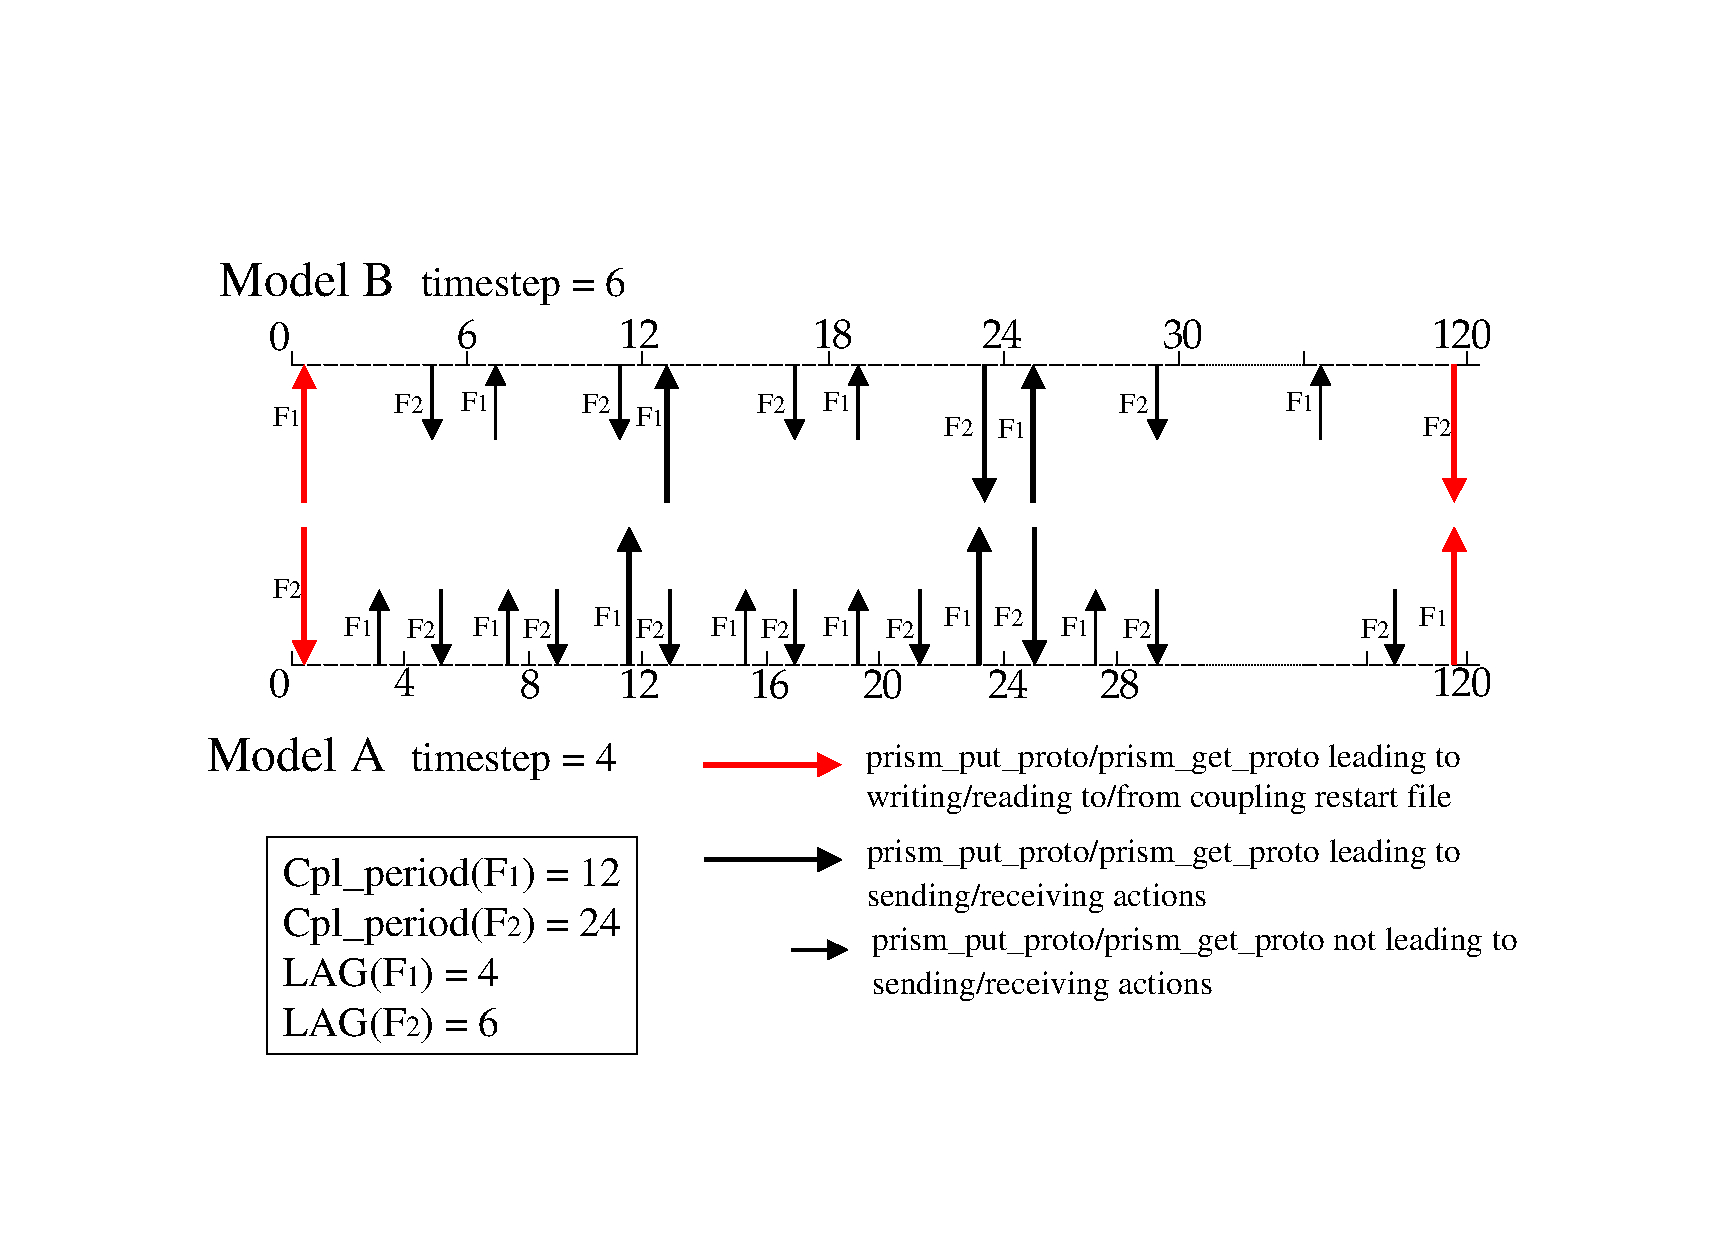
\includegraphics[scale=.6]{fig_lag_concept_1.eps}
\caption{LAG concept first example} 
\label{fig:lag_concept_1}
\end{figure}

  During a coupling timestep, model A receives $F_2$ and then sends $F_1$; its
  timestep length is 4. During a coupling timestep, model B receives $F_1$
  and then sends $F_2$; its timestep length is 6.  $F_1$ and $F_2$
  coupling periods are respectively 12 and 24. If $F_1$/$F_2$ sending
  action by model A/B was used at a coupling timestep to match the
  model B/A receiving action, a deadlock would occur as both models
  would be initially waiting on a receiving action. To prevent this,
  $F_1$ and $F_2$ produced at the timestep before have to be used to
  match respectively the model B and model A receiving actions.

  This implies that a lag of respectively 4 and 6 seconds must be
  defined for $F_1$ and $F_2$. For $F_1$, the {\tt prism\_put\_proto}
  performed at time 8 and 20 by model A will then lead to sending actions
  (as 8 + 4 = 12 and 20 + 4 = 24 which are coupling periods) that
  match the receiving actions performed at times 12 and 24 below the {\tt
  prism\_get\_proto} called by model B.  For $F_2$, the {\tt
  prism\_put\_proto} performed at time 18 by model B then leads to
  a sending action (as 18 + 6 = 24 which is a coupling
  period) that matches the receiving action performed at time 24
  below the {\tt prism\_get\_proto} called by model A.

  At the beginning of the run, as their LAG index is greater than 0,
  the first {\tt prism\_get\_proto} will automatically lead to reading
  $F_1$ and $F_2$ from their coupling restart files. The user
  therefore have to create those coupling restart files for the first
  run in the experiment. At the end of the run, $F_1$
  having a lag greater than 0, is automatically written to its
  coupling restart file below the last $F_1$ {\tt prism\_put\_proto} if the
  {\tt date} + $F_1$ lag equals a coupling time. The analogue is true
  for $F_2$. These
  values will automatically be read in at the beginning of the next
  run below the respective {\tt prism\_get\_proto}.

  \item LAG concept second example

  A second coupling algorithm exploiting the LAG concept is
  illustrated on figure \ref{fig:lag_concept_2}. During its timestep,
  model A receives $F_2$, sends $F_3$ and then $F_1$; its timestep
  length is 6. During its timestep, model B receives $F_1$, receives
  $F_3$ and then sends $F_2$; its timestep length is also 6.  $F_1$,
  $F_2$ and $F_3$ coupling periods are both supposed to be equal to
  12.
 
\begin{figure}
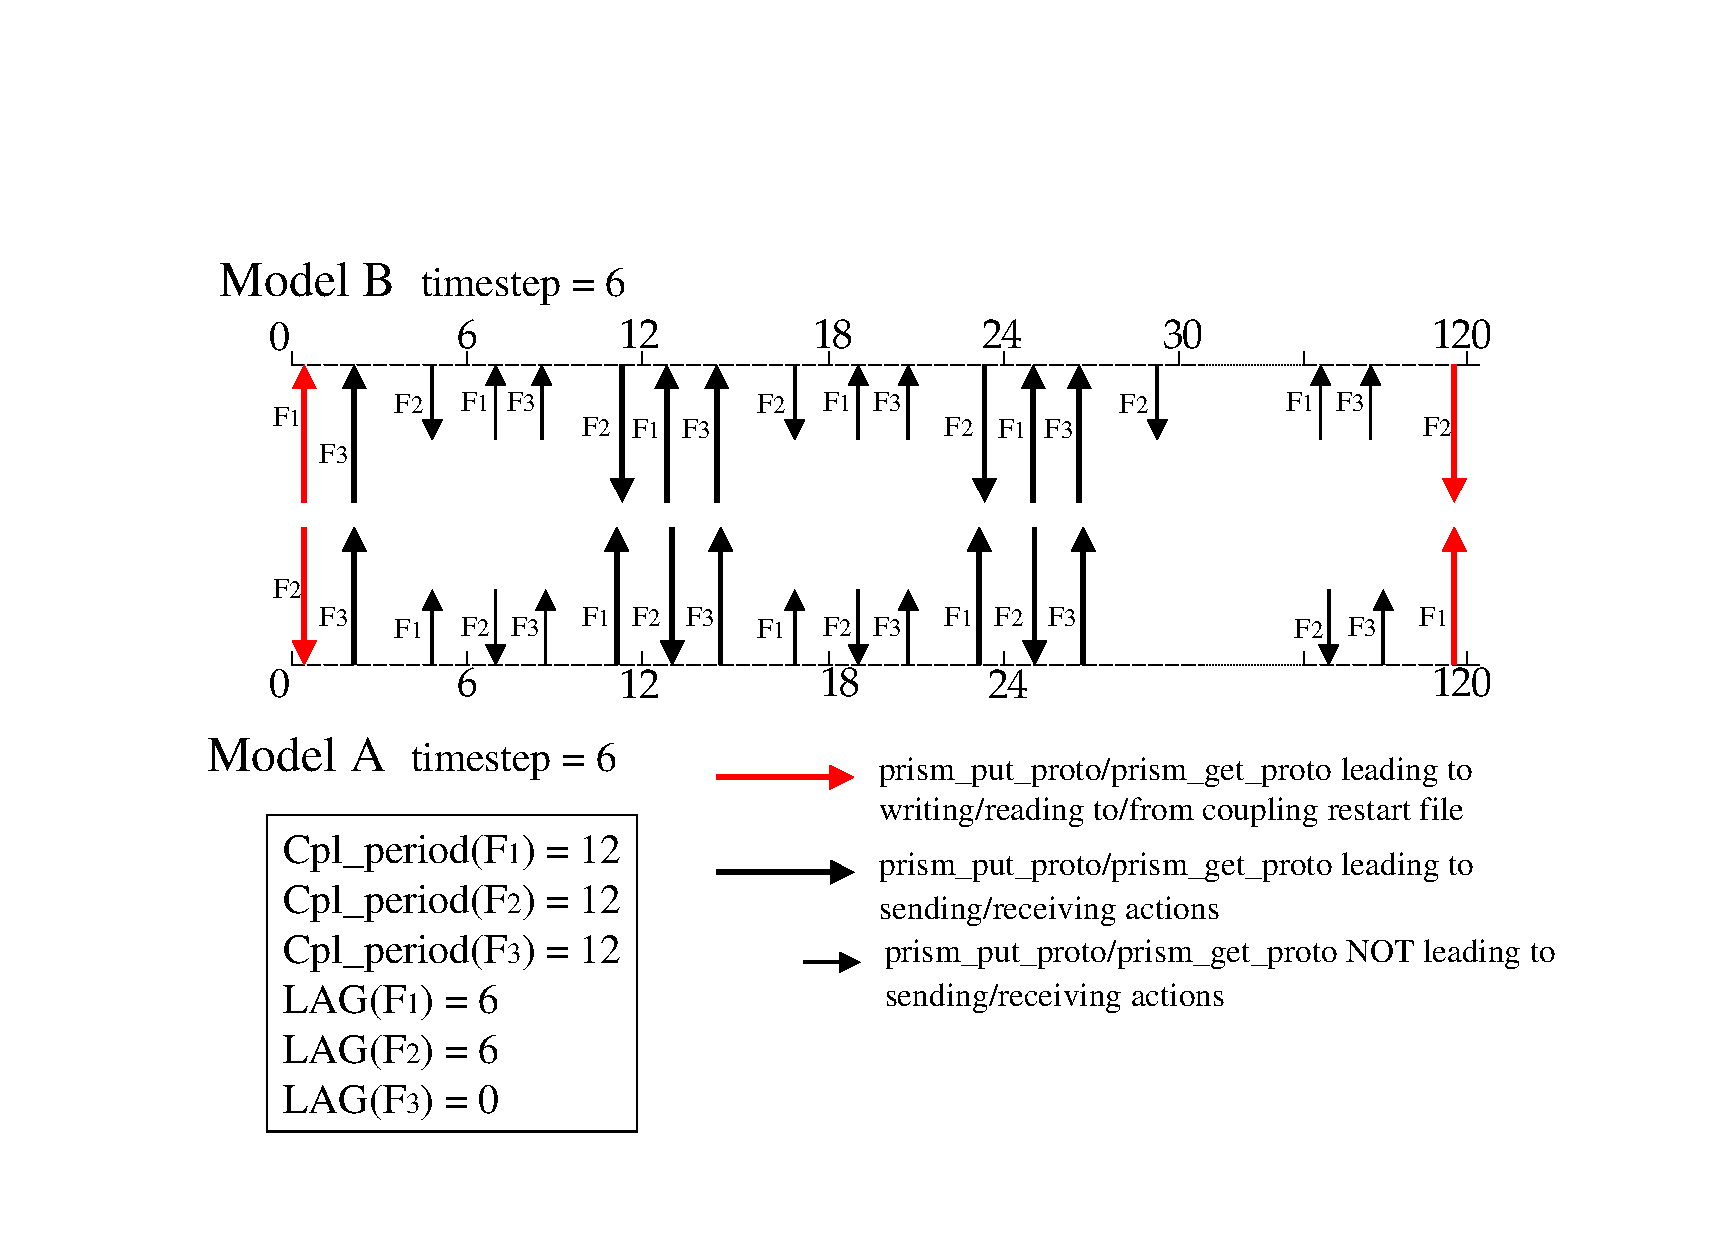
\includegraphics[scale=.6]{fig_lag_concept_2.eps} 
\caption{LAG concept second example} 
\label{fig:lag_concept_2}
\end{figure}

  For $F_1$ and $F_2$ the situation is similar to the first
  example. If $F_1$/$F_2$ sending action by model A/B was used at a
  coupling timestep to match the model B/A receiving action, a
  deadlock would occur as both models would be waiting on a receiving
  action. To prevent this, $F_1$ and $F_2$ produced at the timestep
  before have to be used to match the model A and model B receiving
  actions, which means that a lag of 6 must be defined for both $F_1$
  and $F_2$. For both coupling fields, the {\tt prism\_put\_proto}
  performed at times 6 and 18 by the source model then lead to sending
  actions (as 6 + 6 = 12 and 18 + 6 = 24 which are coupling periods)
  that match the receiving action performed at time 12 and 24 below
  the {\tt prism\_get\_proto} called by the target model.

  For $F_3$, sent by model A and received by model B, no lag
  needs to be defined: the coupling field produced by model A at the
  coupling timestep can be ``consumed'' by model B without causing a
  deadlock situation.

  As in the first example, the {\tt prism\_get\_proto} performed at
  the beginning of the run for $F_1$ and $F_2$, automatically read
  them from their coupling restart files, and the last {\tt
  prism\_put\_proto} performed at the end of the run automatically
  write them to their coupling restart file. For $F_3$, no coupling
  restart file is needed nor used as at each coupling period the
  coupling field produced by model A can be directly ``consumed'' by
  model B.

  We see here how the introduction of appropriate LAG indices results in
  receiving, below the \break {\tt prism\_get\_proto} in the target model,
  coupling fields produced, below the {\tt prism\_put\_proto} by the
  source model, the timestep before; this is, in some coupling
  configurations, essential to avoid deadlock situations.

  \end{enumerate}

\subsection{The sequence concept}
 
To exchange the coupling fields going through OASIS3 main process
(i.e. with status EXPORTED, AUXILARY, or EXPOUT, see section
\ref{sec_namcouple}), in a given order at each coupling timestep, a
sequence index SEQ must be defined for each of them. This is not
required for I/O fields or for coupling fields exchanged directly
between the component models, i.e. with status IGNOUT, INPUT or
OUTPUT. SEQ gives the position of the coupling field in the
sequence.

\begin{figure}
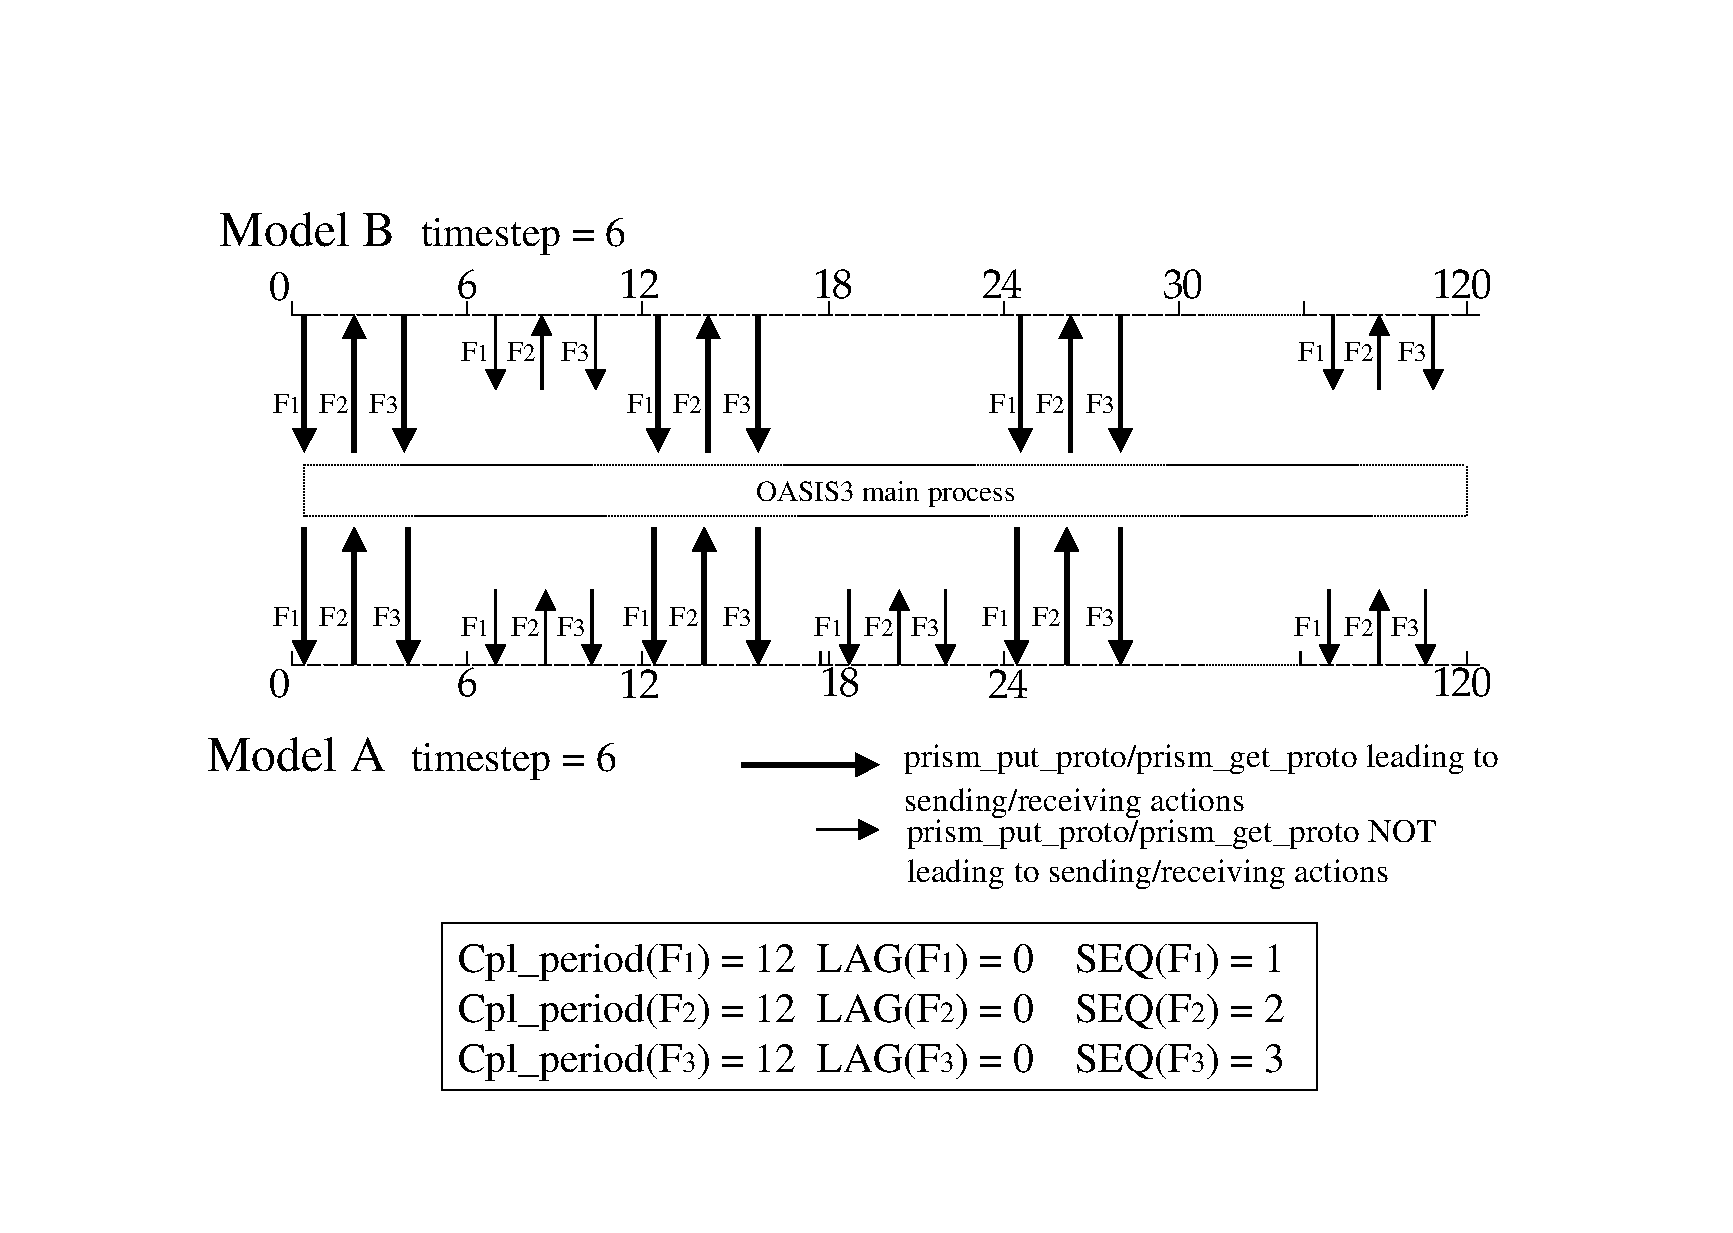
\includegraphics[scale=.6]{fig_seq_concept.eps} 
\caption{The SEQ concept}
\label{fig:seq_concept}
\end{figure}

A coupling algorithm, showing the SEQ concept, is illustrated on
figure \ref{fig:seq_concept}. All coupling field produced by the
source model at the coupling timestep can be ``consumed'' by the
target model at the same timestep without causing any
deadlock situation; therefore, LAG = 0 for all coupling fields.
However, at each coupling timestep, a particular order
of exchange must be respected; $F_1$ must be received by
model A before it can send $F_2$, which in turn must be received by model B
before it can send $F_3$. Therefore, SEQ = 1, 2, 3 must be defined
respectively for $F_1$, $F_2$ and $F_3$. 
As all fields can be consumed at the time they are produced (LAG=0 for
all fields), there no reading/writing from/to coupling restart files.

\subsection{A mix of lag and sequence: the sequential coupled model}
\label{subsubsec_mix}

One can run the same component models simultaneously or sequentially
by defining the appropriate LAG and SEQ indices. In the example
illustrated on figure \ref{fig:mix_seqlag}, the models perform their
{\tt prism\_put\_proto} and {\tt prism\_get\_proto} calls exactly as
in the first lag example above: model A receives $F_2$ and then sends
$F_1$; its timestep length is 4. During a coupling timestep, model B
receives $F_1$ and then sends $F_2$; its timestep length is 6.  $F_1$
and $F_2$ coupling periods are both 12. By defining a LAG index of -8
for $F_1$, the models will now run sequentially.

\begin{figure}
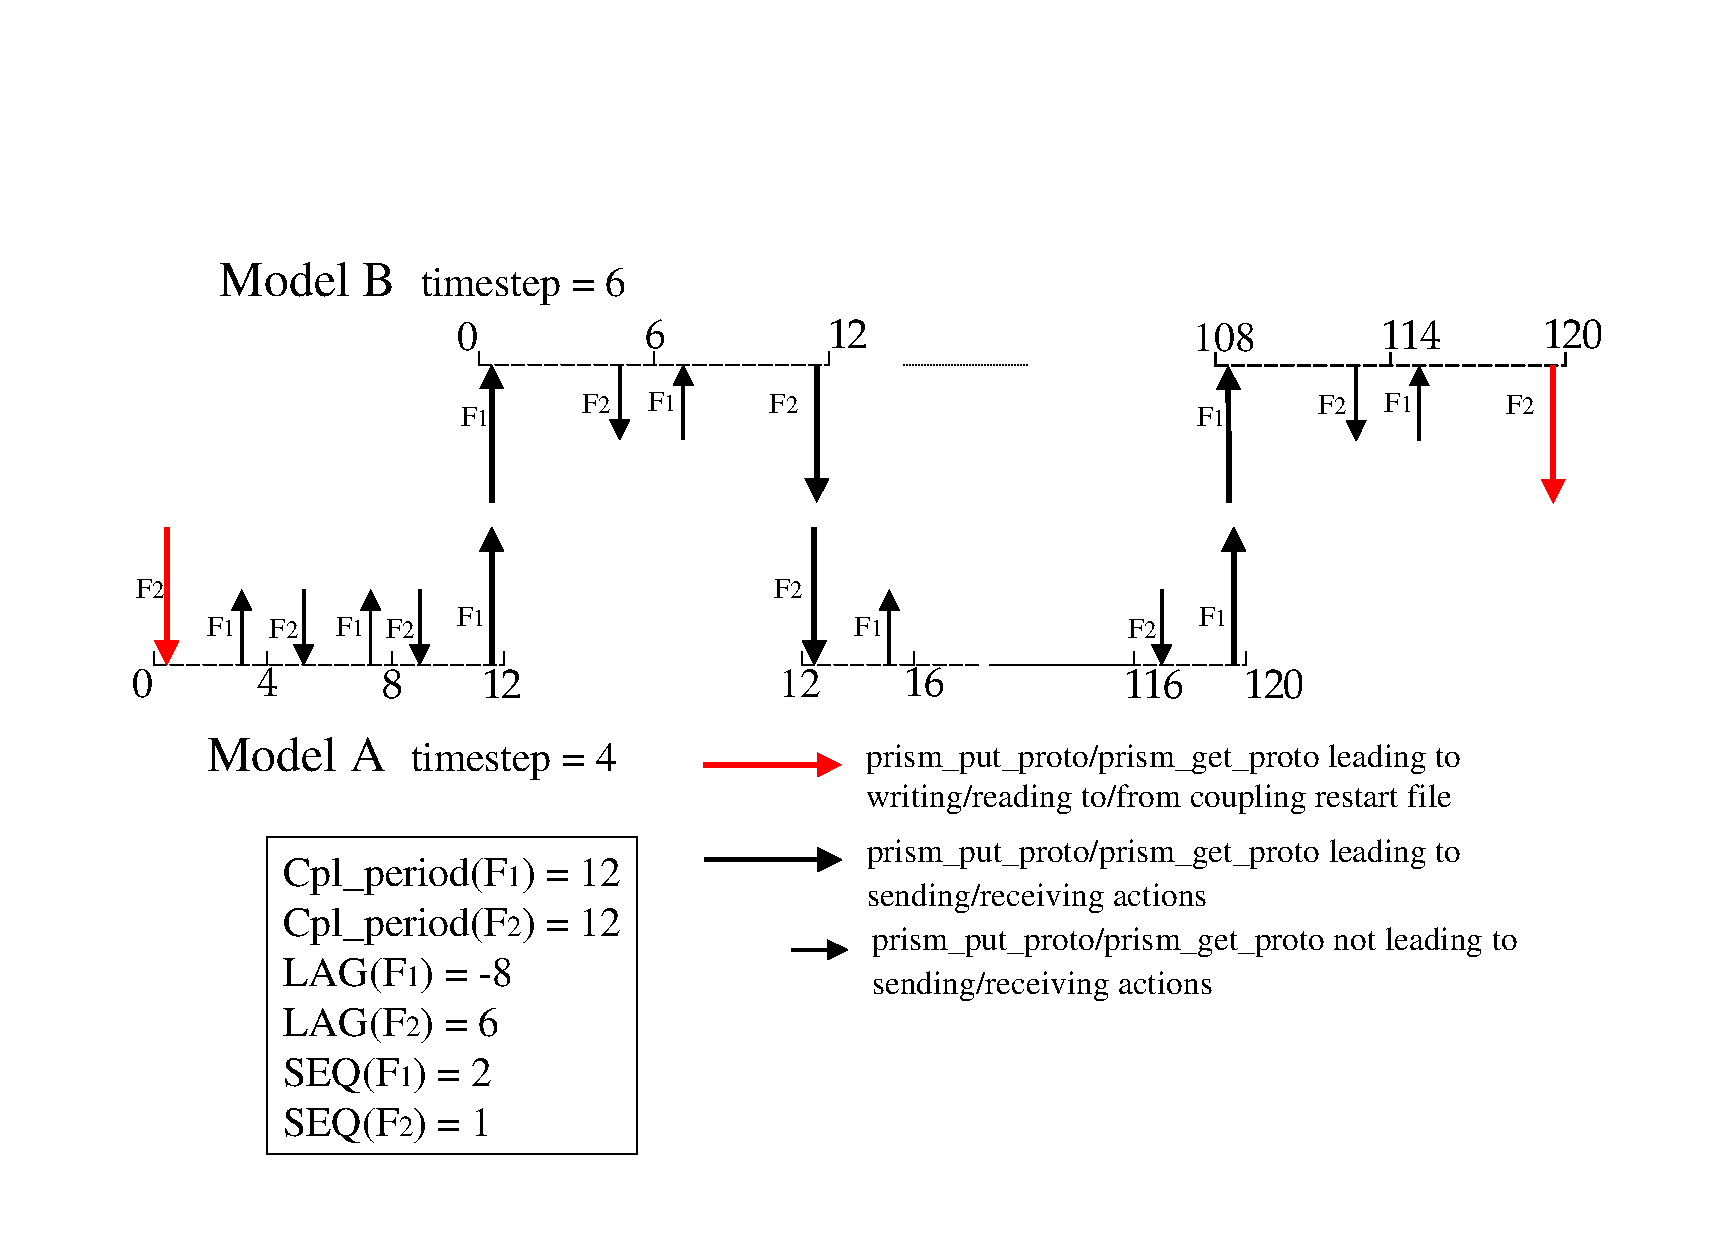
\includegraphics[scale=.6]{fig_mix_seqlag.eps}
\caption{Mix of LAF and SEQ concepts}
\label{fig:mix_seqlag}
\end{figure}

As the LAG for $F_2$ is positive (6), a reading of $F_2$ in its
coupling restart file is automatically performed below the initial
{\tt prism\_get\_proto}. As the LAG for $F_1$ is negative (-8), no
reading from file is performed initially and model B waits; at time 8,
a sending action is effectively performed below model A $F_1$ {\tt
prism\_put\_proto} (as 8 + LAG (-8) = 0 which is the first coupling
timestep) and matches the initial model B $F_1$ {\tt
prism\_get\_proto}. Below the last model A $F_1$ {\tt
prism\_put\_proto} of the run at time 116, a sending action is
effectively performed, as $116 + LAG(-8) = 108$ is a coupling period
(as the LAG is negative, the field is not written to its coupling
restart file). Below the last model B $F_2$ {\tt prism\_put\_proto} of
the run at time 114, a writing of $F_2$ to its restart file is
performed, as $114 + LAG(6) = 120$ is a coupling period and as the LAG
is positive.

If the coupling fields are transformed through OASIS3 main process, it
is important to indicate a sequence index. In fact, at each OASIS3
main process coupling timestep, $F_1$ is necessarily treated after
$F_2$. Therefore, $SEQ(F_1) = 2$ and $SEQ(F_2) = 1$.

\subsection{Mixing sequential and parallel
    runs using {\tt prism\_put\_restart\_proto}}

In the example illustrated on figure \ref{restart_ex}, the models
run sequentially for the first run only and then run
simultaneously. For the first run, the LAG and SEQ indices must be
defined as in section \ref{subsubsec_mix}.  After the first run, the
situation is similar to the one of section \ref{subsub_lag}, and
positive LAG must be defined for $F_1$ and $F_2$. As their lag is
positive, their corresponding first {\tt prism\_get\_proto} will
automatically lead to reading $F_1$ and $F_2$ from coupling restart
files.  In this case, model A has to write $F_1$ to its restart file
explicitly by calling {\tt prism\_put\_restart\_proto} (illustrated
on the figure by an orange arrow) at the end of the first run; in
fact, $F_1$ lag being then negative, such writing is not automatically
done below the last {\tt prism\_put\_proto} of the first run.


\begin{figure}
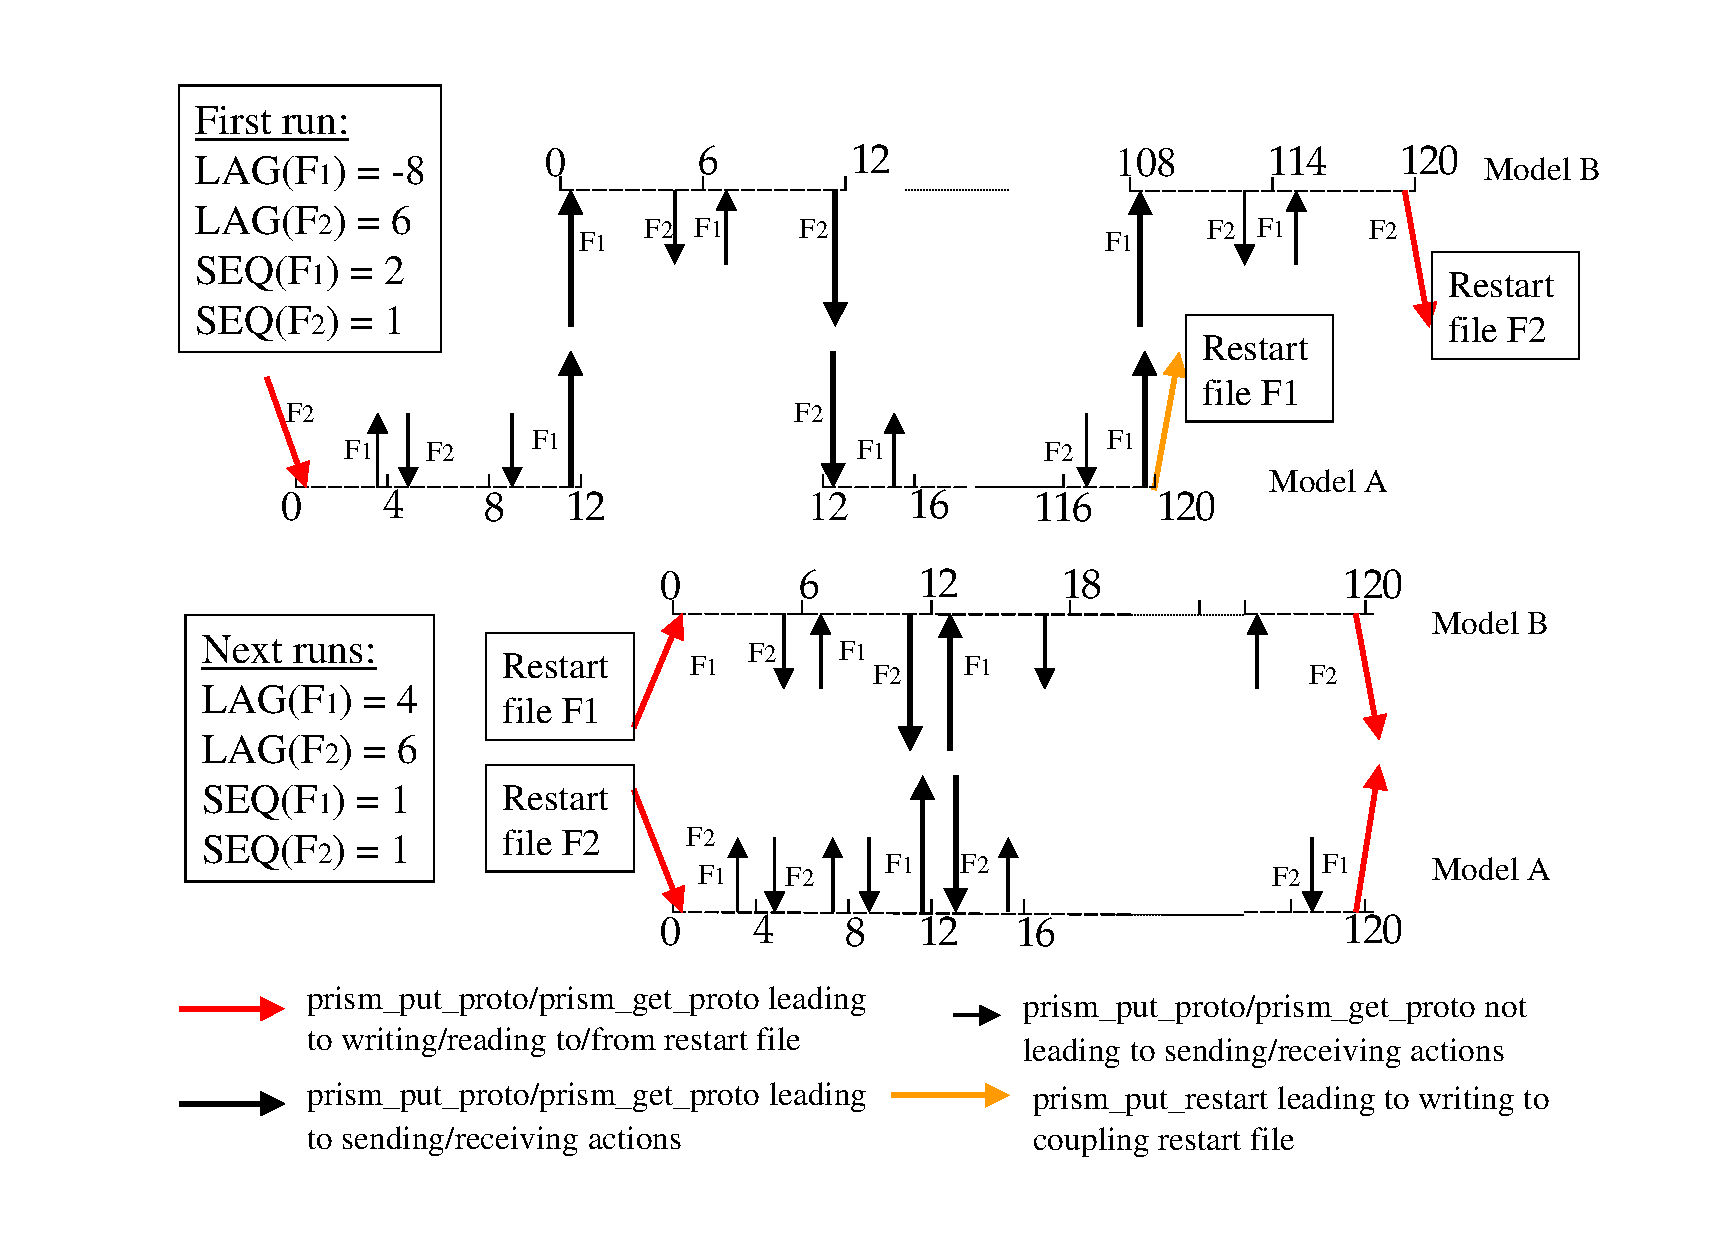
\includegraphics[scale=.6]{restart_example.eps} 
\caption{An example using prism\_put\_restart\_proto}
\label{restart_ex}
\end{figure} 

%section{PRISM System Model Interface for the CLIM/MPI2-MPI1
%communication technique (PSMILe V.0)}
%section{Model\_interfacing} 
